%\let\textcircled=\pgftextcircled
\chapter{Trajectory integration}
\label{chap:trajectory_integration}

Initially I coded both the square, the trapezoid and the parabola method, to analyze better suited my necessities. \cite{casciola} The last one, from now on, will be called PaIS (Parabola integrator for Irregular Spaced data),  \\
A quadrature formula of grade $n$ provides the exact integral value of a polynomial of grade $\leq n$, which means that it isn't always necessary to use a formula with a high grade. \\
\\
\justify
I verified experimentally the difference in error between integration methods by creating synthetic trajectories.
\begin{figure}[H]
\centering
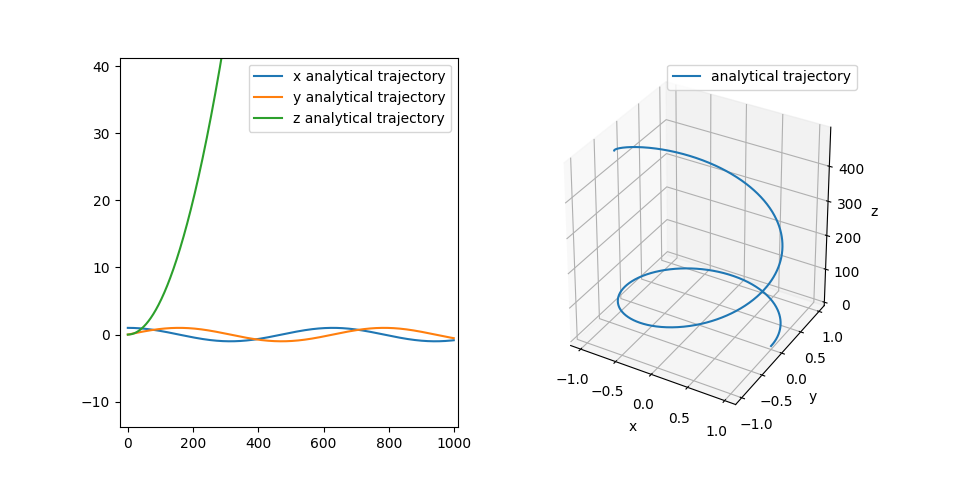
\includegraphics[scale=0.6]{spring.png}
\caption{Trajectory created to evaluate integration error}
\end{figure}
\justify
then I compared the integrated one with the analytical.
\begin{figure}[H]
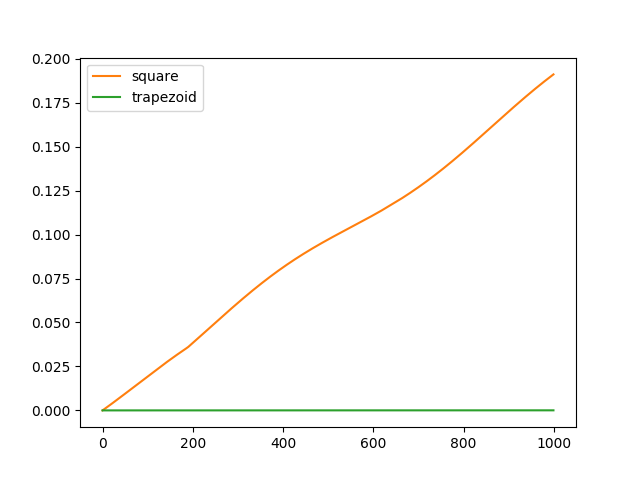
\includegraphics[width=\textwidth/2]{square_vs_trapezoid.png}
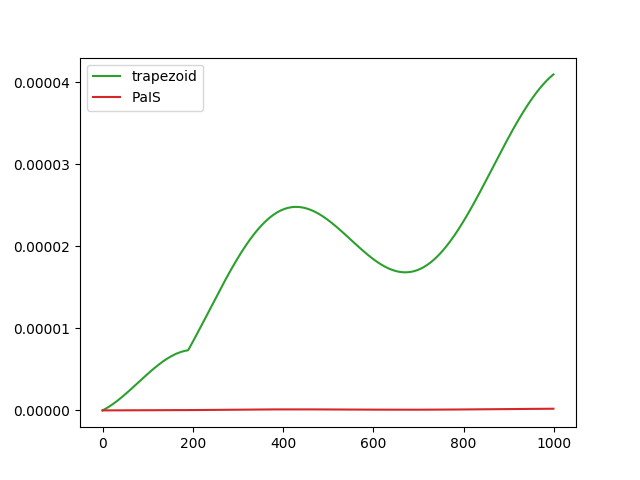
\includegraphics[width=\textwidth/2]{trapezoid_vs_PaIS.png}
\caption{Absolute error from analytical trajectory}
\end{figure}

\justify
Numpy offers a compact way to write operation even on large arrays. This is for example the trapezoid method in one line.

\begin{lstlisting}[language=Python,frame=single,basicstyle=\footnotesize]
def trapz_integrate_delta(times, vector):
    return (((vector[:,:-1] + vector[:,1:]) * (times[1:]-times[:-1])) * 0.5).cumsum()
\end{lstlisting}

Difference between PaIS and trapezoid can be seen after integrating for 40 thousands steps.
\begin{figure}[H]
\centering
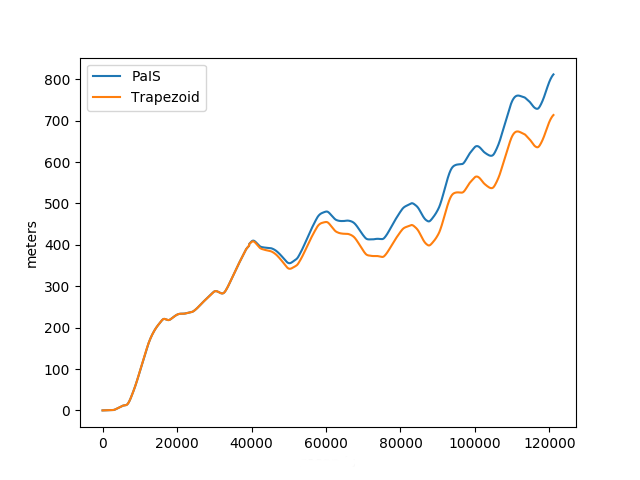
\includegraphics[scale=0.6]{trapezoid_vs_Pais_real_world.png}
\caption{Difference between trapezoid and PaIS method on real world data}
\end{figure}

\justify
I decided to use the PaIS integrator because measures in discrete time produce a function $C^0$, while physics quantities of a vehicle in continuous time are at least $C^1$, 
\justify
But still the error was too large, the integrated trajectory diverges after some time by moving away too much from the real trajectory.
So I improved integrated trajectory using GNSS data, which is more precise but has lower frequency and has difficulties on finding orientation. In this way, the output trajectory benefits from both measures, using their respective advantages and reducing each other disadvantage. Accelerometer and gyroscope are really good in small time frames, but due to integrated quantities have precision problems on long time spans. On the other hand commercial GNSS sensors don't have very precise positioning but they keep working steady for much times.
I started from resetting the integrated position to the GNSS one every $t$ times, but this was causing an edgy and irregular behavior that wasn't realistic.
I proceeded to implementing a contiguous weighted average, so that GNSS component is always present in the output trajectory but its impact is limited. Especially when GNSS signal is low,the position completely wrong, in the order of tens of meters. Giving a low weight to GNSS, like 1 on 99, avoid problems caused by low signals but still helps with correcting numerical integration error.

\begin{figure}[H]
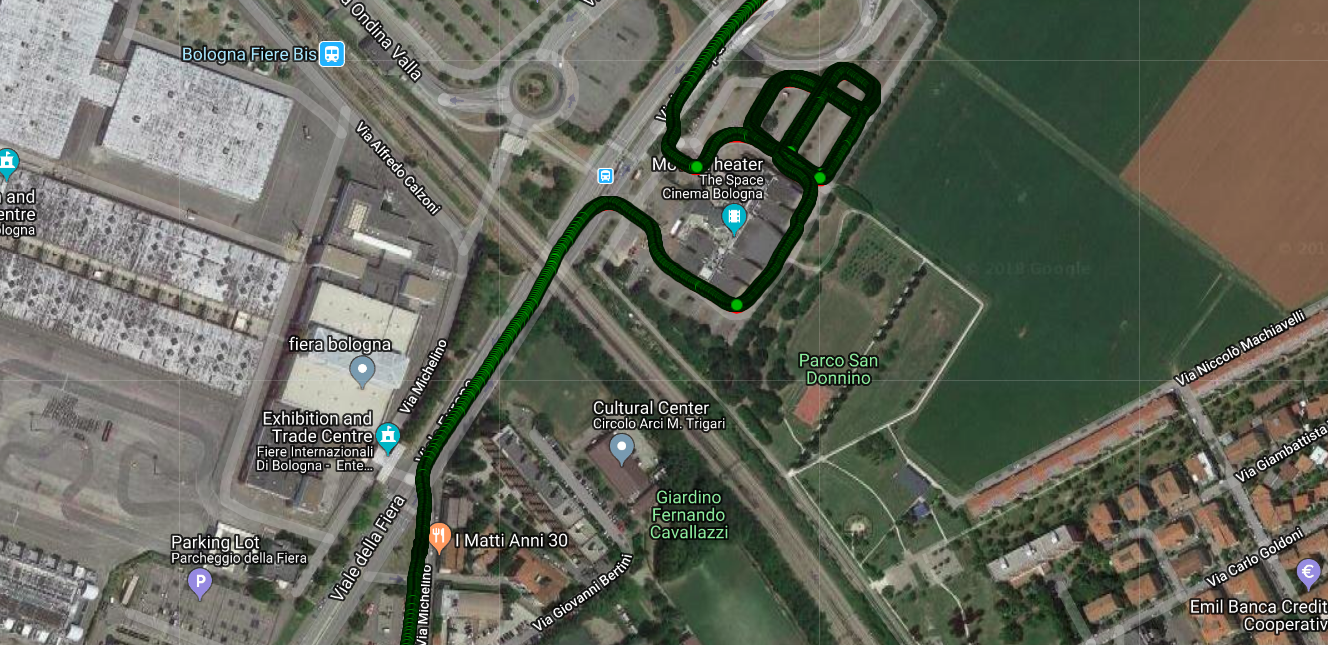
\includegraphics[width=\textwidth]{parking_map.png}
\caption{Path traveled by a car with a box installed, in a Bologna parking}
\end{figure}
\begin{figure}[H]
\centering
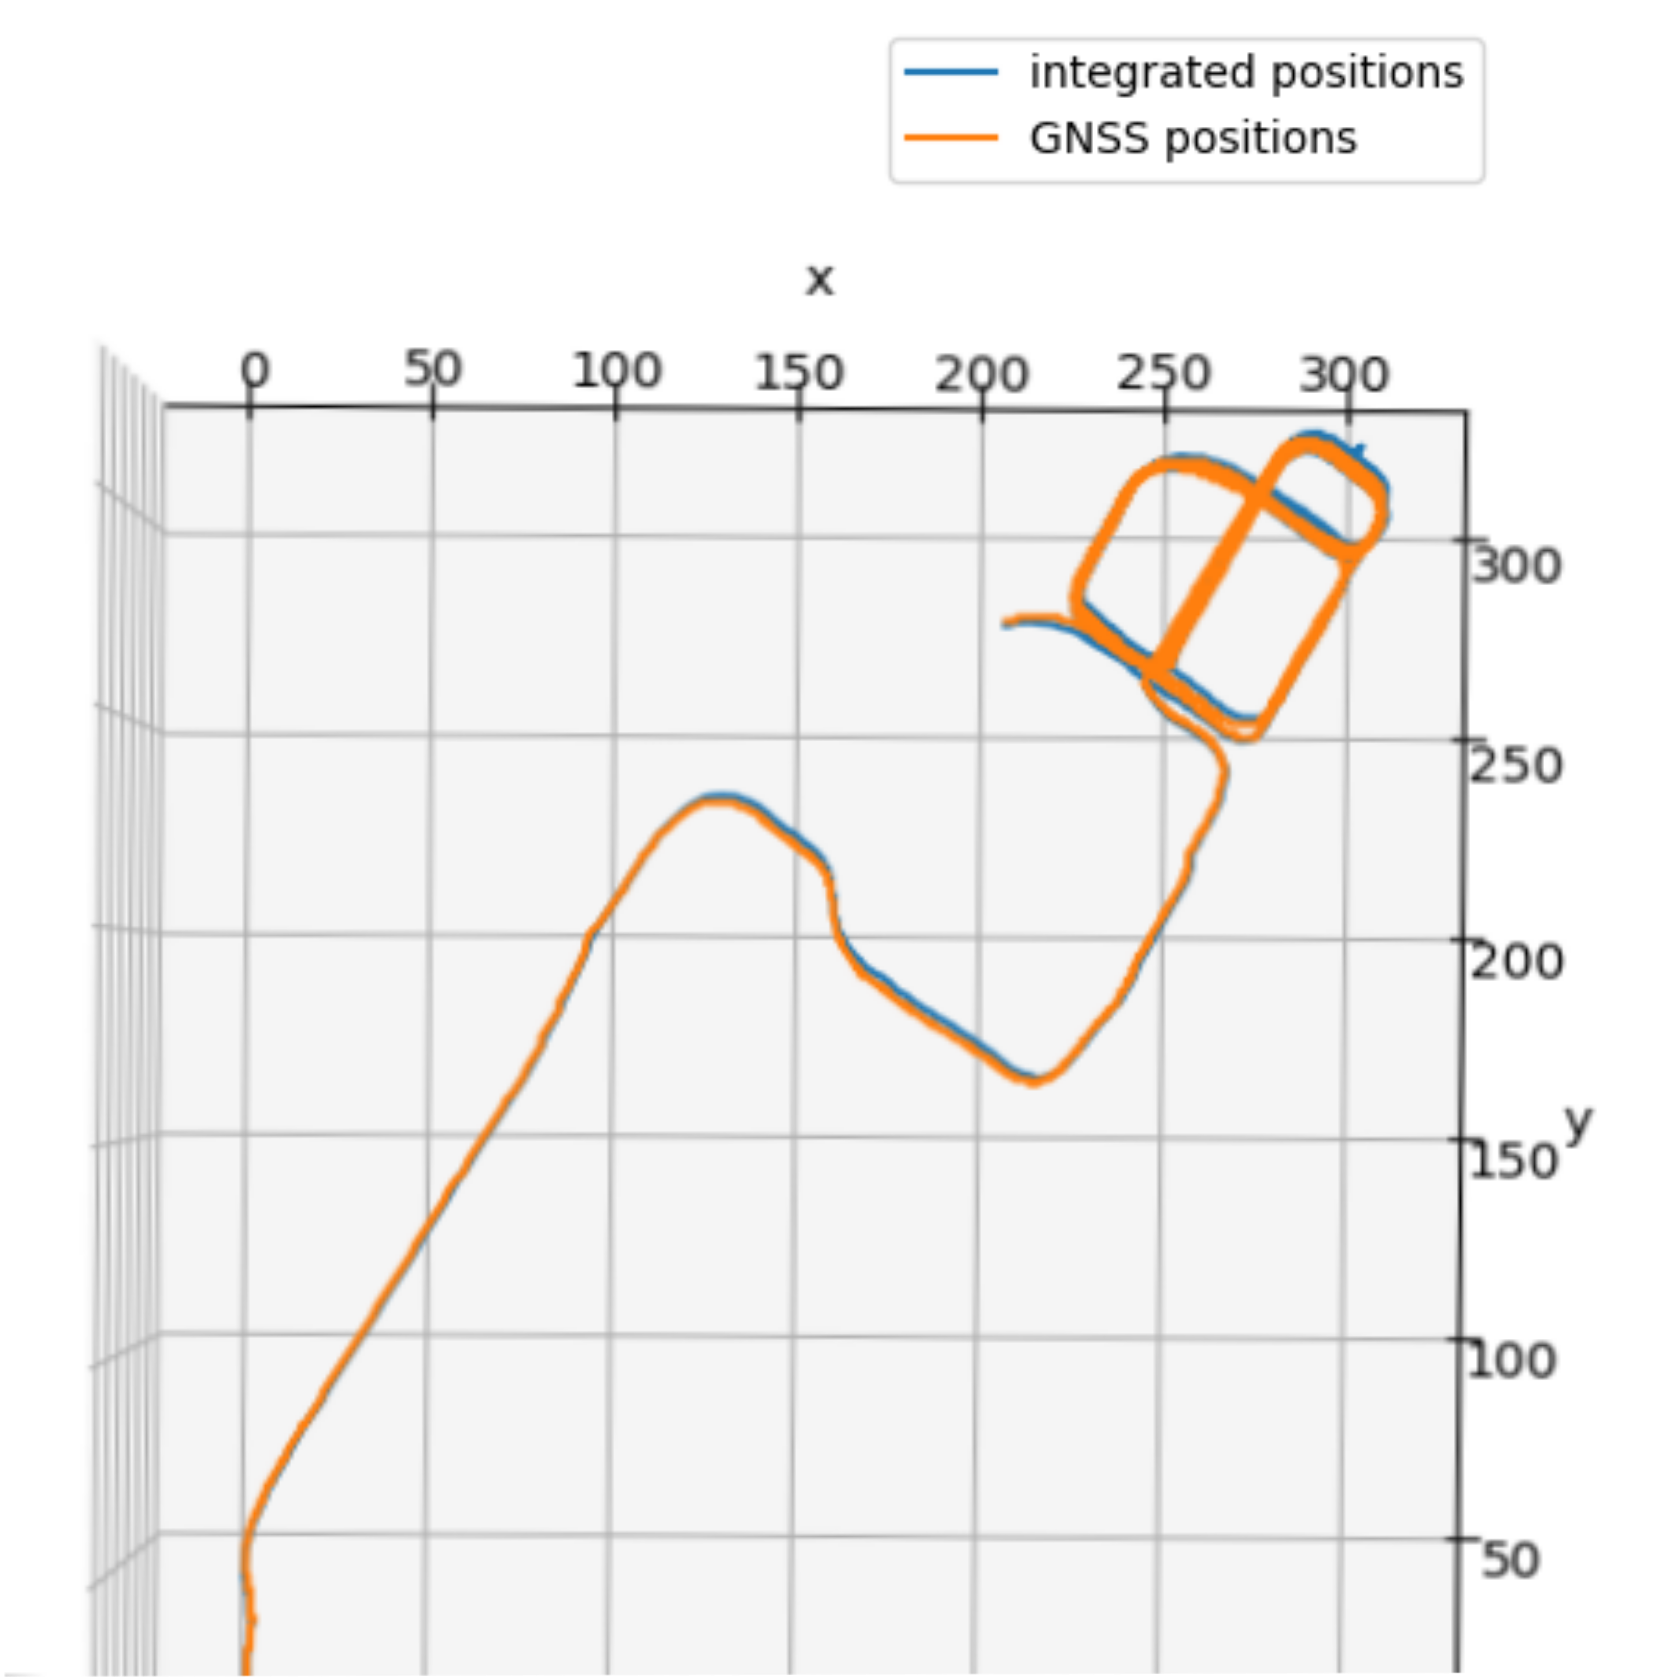
\includegraphics[scale=0.6]{parking_3d.png}
\caption{The same path from data registered by sensors and elaborated by the program}
\end{figure}
\begin{figure}[H]
\centering
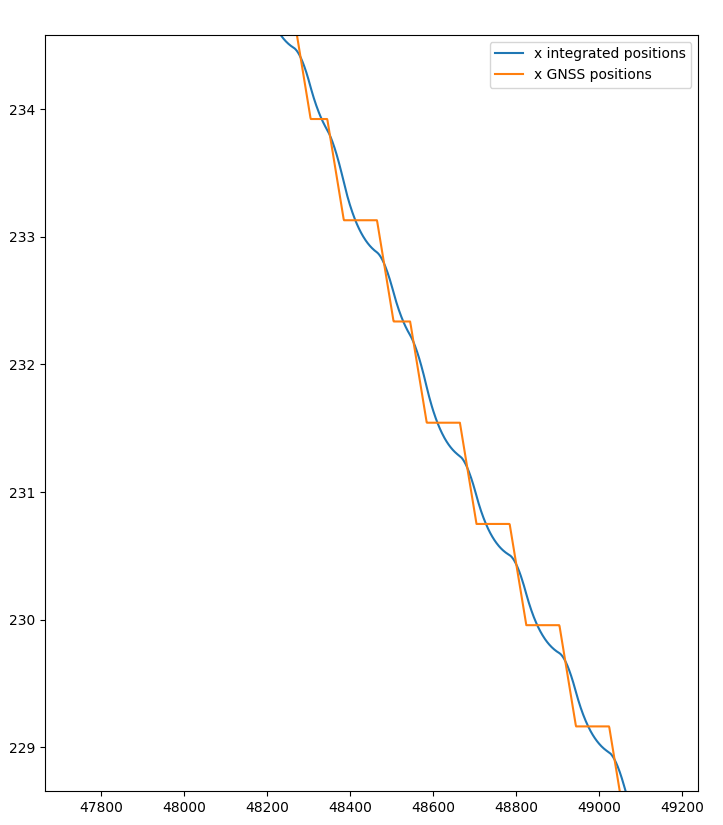
\includegraphics[width=\textwidth/2]{smooth.png}
\caption{Particular showing smoothness of integrated trajectory in respect of GNSS one}
\end{figure}

\begin{figure}[H]
\centering
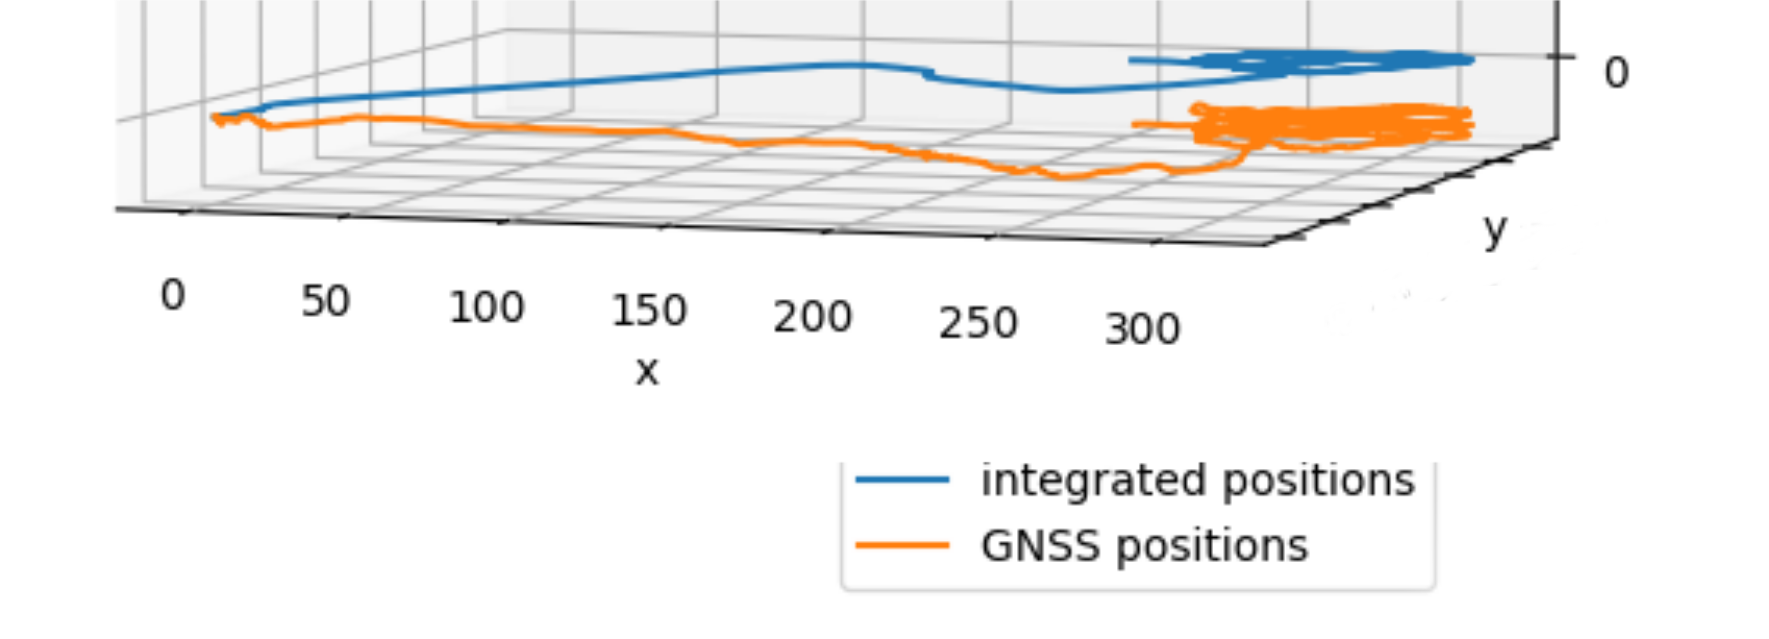
\includegraphics[width=0.8\textwidth]{parking_3d_z_different.png}
\caption{Note that GNSS and integrated path are distant on vertical axis. This is because altitude from GNSS system is extremely unreliable to determine vertical position. In my algorithm i Decided to neglect this information and only use the integrated accelerometer information.}
\end{figure}


